\documentclass[]{spie}  %>>> use for US letter paper
%\documentclass[a4paper]{spie}  %>>> use this instead for A4 paper
%\documentclass[nocompress]{spie}  %>>> to avoid compression of citations

\renewcommand{\baselinestretch}{1.0} % Change to 1.65 for double spacing
 
\usepackage{amsmath,amsfonts,amssymb}
\usepackage{graphicx}
\usepackage[colorlinks=true, allcolors=blue]{hyperref}

\title{Simulating the LSST OCS for Conducting Survey Simulations Using the LSST Scheduler}

\author[a]{Michael A. Reuter*}
\author[b]{Kem H. Cook}
\author[a]{Francisco Delgado}
\author[a]{Catherine E. Petry}
\author[c]{Stephen T. Ridgway}
\affil[a]{LSST, 950 N Cherry Ave, Tucson, AZ USA}
\affil[b]{Cook Astronomical Consulting, San Ramone, CA USA}
\affil[c]{National Optical Astronomy Observatory, 950 N Cherry Ave, Tucson, AZ USA}

%\authorinfo{Further author information: (Send correspondence to M.A.R.)\\M.A.R.: E-mail: mareuter@lsst.org, Telephone: 1 520 318 8204}

% Option to view page numbers
\pagestyle{empty} % change to \pagestyle{plain} for page numbers   
\setcounter{page}{301} % Set start page numbering at e.g. 301
 
\begin{document} 
\maketitle

\begin{abstract}
The Operations Simulator was used to prototype the LSST Scheduler. Currently, the Scheduler is being developed separately to interface with the LSST Observatory Control System (OCS).  A new Simulator is under concurrent development to adjust to this new architecture.  This requires a package simulating enough of the OCS to allow execution of realistic schedules. This new package is called the Simulated OCS (SOCS). In this paper we will detail the SOCS construction plan, package structure, LSST communication middleware platform use, provide some interesting use cases that the separated architecture allows and the software engineering practices used in development.
\end{abstract}

% Include a list of keywords after the abstract 
\keywords{LSST, simulations, observing strategy}

\section{INTRODUCTION}
\label{sec:intro}  % \label{} allows reference to this section

In both research and development phase of the LSST project prior to the construction award in August 2014 and the subsequent years afterwards saw the successful development and testing of the Operations Simulator (OpSim) \cite{2014SPIE.9149E..0GD}\cite{2014SPIE.9150E..15D}\cite{2013AAS...22124703S}\cite{2010SPIE.7737E..0ZR}\cite{2010AAS...21540105K}\cite{2009AAS...21346004C}\cite{2007AAS...21113703P}\cite{2006SPIE.6270E..1DD}\cite{2006AAS...209.8604P}\cite{2005AAS...207.2626C}\cite{2004AAS...20510809C} . OpSim contains the prototype version of the LSST Scheduler and this has been tuned to produce the current LSST baseline survey as well as alternate survey strategies\cite{Cook_SPIE2016}. When LSST begins operations, it will require the Scheduler to perform the duties of determining the next targets to observe. The current state of OpSim has the Scheduler entwined within the code based. The LSST project decided to separate the Scheduler\cite{Delgado_SPIE2016} into its own code base so that an effective deliverable can be provided. The Scheduler is required to interface with the LSST's Observatory Control System (OCS)\cite{Daly_SPIE2016} via the Data Distribution Service (DDS) which is behind the LSST communication middleware\cite{Mills_SPIE2016} project. DDS is a publish/subscribe system in common use for communication between
components of complex systems. In order to continue running simulations with the refactored Scheduler, a new harness is being created that utilizes the same DDS infrastructure to communicate with the Scheduler. This new project is called the Simulated Observatory Control System (SOCS). SOCS is not a high fidelity simulation of the entire OCS, but just enough of it to get the Scheduler to complete an entire survey. The combination of SOCS and the Scheduler is still collectively called the OpSim version 4 whereas the older Operations Simulator is now referred to as OpSim version 3.

\begin{figure} [ht]
  	\begin{center}
  		\begin{tabular}{c} 
  			\includegraphics[height=4cm]{Opsimv3.png}
  			\includegraphics[height=4cm]{Opsimv4.png}
  		\end{tabular}
  	\end{center}
  	\caption[What is this?] 
  	{ \label{fig:opsim} 
  		The left figure schematically shows the operational bounding box for OpSim version 3. This clearly indicates the buried nature of the Scheduler within the confines of OpSim. The right figure schematically shows the operational bounding box for OpSim version 4. This shows the newly separated nature of the two component which allow for development and usage flexibility.}
\end{figure} 

\section{CONSTRUCTION}
\label{sec:construction}

Since SOCS and the Scheduler have intertwined functionality, the developed construction plans are tightly coupled. 

\section{DESIGN}

\begin{figure} [ht]
\begin{center}
\begin{tabular}{c}
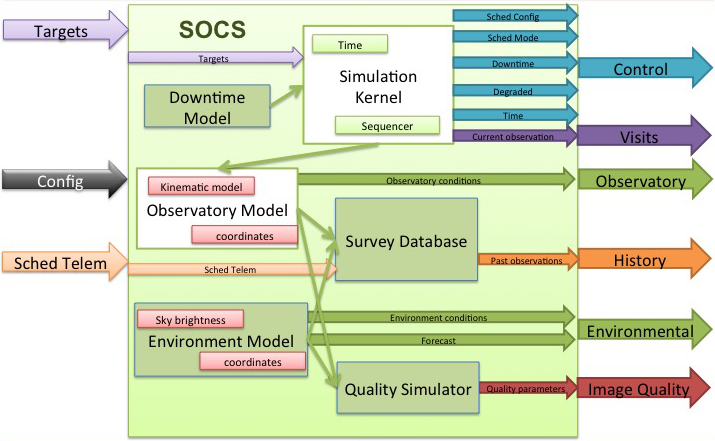
\includegraphics[height=5cm]{CompArch.png}
\end{tabular}
\end{center}
\caption[example]
{ \label{fig:comparch} 
This diagram shows the block level components for the SOCS design as well as the information flow both internal and external to SOCS.}
\end{figure}

\begin{figure} [ht]
	\begin{center}
		\begin{tabular}{c}
			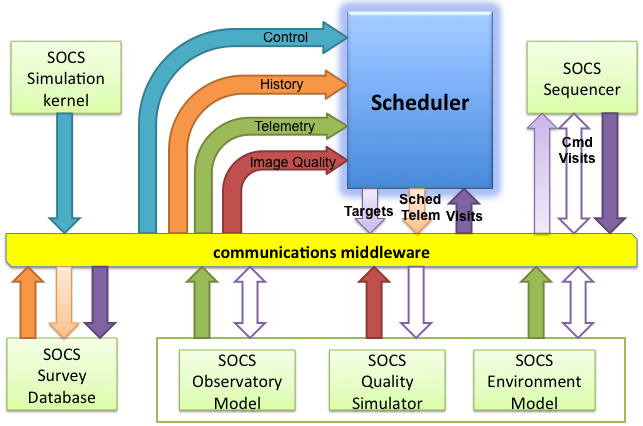
\includegraphics[height=5cm]{CommFlow.png}
		\end{tabular}
	\end{center}
	\caption[example]
	{ \label{fig:commflow} 
		This diagram shows the DDS communication pathways between the SOCS and Scheduler systems.}
\end{figure}

Figure~\ref*{fig:commflow} is an exact replica of a diagram showing the interaction of the Scheduler and the OCS with SOCS simulating OCS functions. The job of SOCS is to provide all of the needed inputs to the Scheduler shown in this diagram. Central to this diagram is the communications middleware, which currently is DDS. The details of this interface are described in the Scheduler interface document. Key to the design of SOCS is the ability to simulate a survey either deterministically or with stochastic variation in a variety of outputs. This is needed to understand the behavior of simulated surveys when the Scheduler is not provided completely accurate environmental data due to rapid variation in the environment, and also when the Scheduler’s telescope model is not a completely accurate model of the real telescope.

\section{SOFTWARE ENGINEERING}

OpSim version 3 had a document detailing all of the functional and performance requirements for the developed system which included those for the Scheduler. The factorization of OpSim version 3 into the SOCS and Scheduler components necessitated a factorization of the requirements document into one for each resulting system. The SOCS requirements document was adjusted to account for the new role as the hardness for driving the Scheduler and placed under LSST project level change control.

A development plan for SOCS was created containing incremental releases, with a specific set of capabilities and validation activities for each one. This plan is captured in JIRA\cite{JIRA} release epics and described at a high level in Primavera PMCS. The plan is coordinated with the release timeline of the Scheduler due to their heavy interdependence.

The detailed construction plan is also described in JIRA epics relating to each release epic, keeping track of individual tasks that mark the way to each release. The tracking the development process uses the LSST variant of Agile Softwa development\cite{Kantor_SPIE2016}. The JIRA plan, releases, milestones and tasks are used periodically to report back to PMCS and to compute EVM, and organize the work of the development team.

The SOCS code is kept in a Github\cite{GitHub} git repository, following coding standards from Data Management and Systems Engineering Simulations about templates, interfaces, coding and unit tests. The SOCS code follows the basic tenants of the Test Driven Design philosophy of software development. TDD requires unit tests to be run during the implementation process at a fairly high frequency to uncover issues quickly. The baseline science survey configuration is also kept with the SOCS Github repository. 

More importantly, each SOCS release is integrated and tested with the LSST Scheduler and the combined efforts from both the Telescope and Site and Systems Engineering Simulations teams. The capabilities of SOCS to drive the Scheduler for implementing the LSST survey are validated with specialized tools (MAF) and the participation of the science collaborations.

\section{USE CASES}

The separation of the Scheduler from the simulation harness allows for efficient development. This means only one code base has to be maintained to serve the separate systems (OCS and SOCS). This separated approach and the use of a standard communication framework allow for some interesting use cases with respect to the SOCS/Scheduler combination. Both cases are predicated off the fact the configuration of the Scheduler that is running the LSST during operations can be injected into a new instance of the Scheduler. The new instance can be driven by SOCS to perform different scenarios while leaving the operating Scheduler unaffected. One scenario is advancing the Scheduler through a given time window in order to publish a list of targets that the LSST will visit within the caveats of environmental and instrumental conditions. Another scenario is to take the current Scheduler state and fast forward through the remaining survey to evaluate the efficiency based off the current progress. This mechanism can also be used to evaluate alternate scenarios for the survey, such as new proposals, proposals being finished or alternate configuration parameters.

\section{SUMMARY}

\acknowledgments % equivalent to \section*{ACKNOWLEDGMENTS}       

Financial support for LSST comes from the National Science Foundation (NSF) through Cooperative Agreement No. 1258333, the Department of Energy (DOE) Office of Science under Contract No. DE-AC02-76SF00515, and private funding raised by the LSST Corporation. The NSF-funded LSST Project Office for construction was established as an operating center under management of the Association of Universities for Research in Astronomy (AURA).  The DOE-funded effort to build the LSST camera is managed by the SLAC National Accelerator Laboratory (SLAC).    

% References
\bibliography{SimObsConSysSPIE991183} % bibliography data in report.bib
\bibliographystyle{spiebib} % makes bibtex use spiebib.bst

\end{document} 
